\documentclass[11pt]{article}
\usepackage[utf8]{inputenc}	% Para caracteres en español
\usepackage{amsmath,amsthm,amsfonts,amssymb,amscd}
\usepackage{multirow,booktabs}
\usepackage[table]{xcolor}
\usepackage{fullpage}
\usepackage{lastpage}
\usepackage{enumitem}
\usepackage{fancyhdr}
\usepackage{mathrsfs}
\usepackage{wrapfig}
\usepackage{setspace}
\usepackage{calc}
\usepackage{multicol}
\usepackage{cancel}
\usepackage{float}
\usepackage{physics}
\usepackage[retainorgcmds]{IEEEtrantools}
\usepackage[margin=1cm]{geometry}
\usepackage{amsmath}
\newlength{\tabcont}
\setlength{\headheight}{14pt}
\setlength{\parindent}{0.0in}
\setlength{\parskip}{0.05in}
\usepackage{empheq}
\usepackage{framed}
\usepackage[most]{tcolorbox}
\usepackage{xcolor}
\usepackage[version=3]{mhchem}
\usepackage[english]{babel}
\usepackage[utf8]{inputenc}
\usepackage{graphicx}
\usepackage[colorinlistoftodos]{todonotes}
\usepackage{mdframed}

\colorlet{shadecolor}{orange!15}
\parindent 0in
\parskip 12pt
\geometry{margin=1in, headsep=0.45in}
\theoremstyle{definition}
\newtheorem{defn}{Definition}
\newtheorem{reg}{Rule}
\newtheorem{exer}{Exercise}
\newtheorem{note}{Note}
\begin{document}
\setcounter{section}{2}
%\setcounter{subsection}{}
\title{Problem Set 12}

%==============================================================
%\thispagestyle{empty}
\pagestyle{fancy}
\fancyhf{}
\rhead{Physics 180}
\chead{Problem Set 12}
\lhead{Olyn D. Desabelle}
\rfoot{Page \thepage}

\begin{center}
{\LARGE \bf Problem Set 12}\\
%{\large Physics 180}\\
%Olyn D. Desabelle
\end{center}

%==============================================================
\begin{figure}[H]
    \centering
    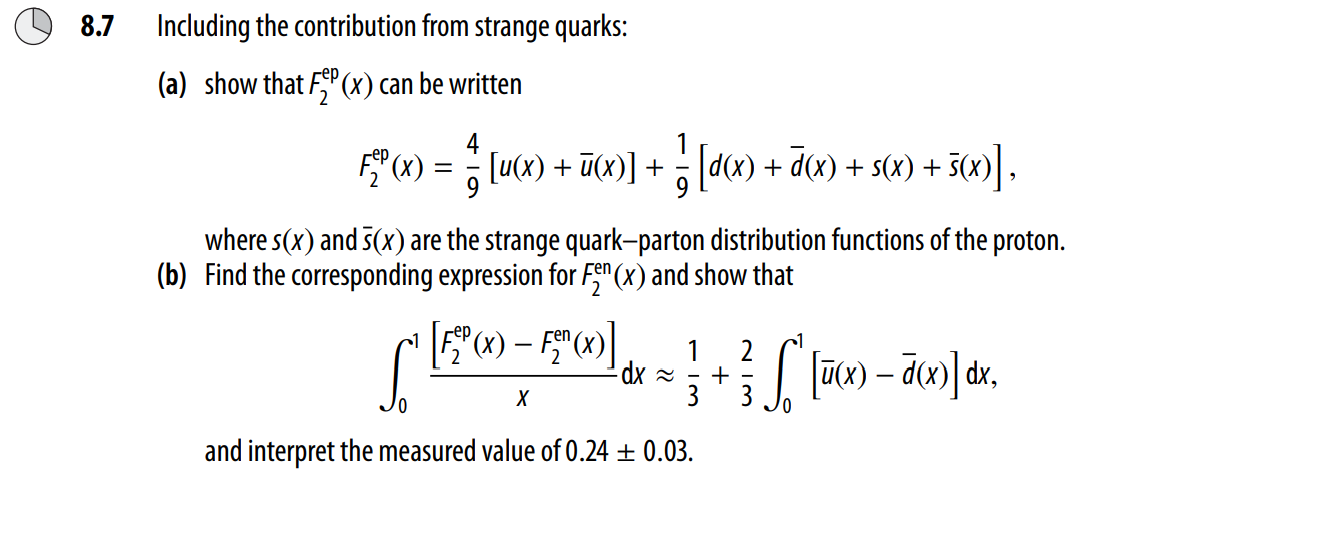
\includegraphics[scale = 0.4]{8.7.png}
\end{figure}

\underline{a)}

Equation (8.24) of Thomson gives the expression for the structure function $F_{2}^{\text{ep}}(x)$:

\begin{align}
    F_{2}^{\text{ep}}(x) &= x \sum_{i} Q_i^2q_i^{\text{p}}\\
    %&\approx x\left( \frac{4}{9} u^{\text{p}}(x) + \frac{1}{9}d^{\text{p}}(x) + \frac{4}{9} u^{-\text{p}}(x) + \frac{1}{9} d^{-\text{p}}(x) \right)
\end{align}

Equation (8.25) expands this with the contributions of the up-, down-, anti-up-, and anti-down parton distribution functions. 

\begin{align}
    F_{2}^{\text{ep}}(x) &= x \sum_{i} Q_i^2q_i^{\text{p}}\\
    &\approx x\left( \frac{4}{9} u^{\text{p}}(x) + \frac{1}{9}d^{\text{p}}(x) + \frac{4}{9} u^{-\text{p}}(x) + \frac{1}{9} d^{-\text{p}}(x)  \right)
\end{align}

this may be rewritten in a more simplified way such that:

\begin{align}
    u^{\text{p}}(x) \equiv u(x) \;\;\; &\text{ and }\;\;\; d^{\text{p}}(x) \equiv d(x)\\
    u^{-\text{p}}(x) \equiv \bar{u}(x) \;\;\; &\text{ and }\;\;\; d^{-\text{p}}(x) \equiv \bar{d}(x)\\
\end{align}

giving us:

\begin{align}
    F_{2}^{\text{ep}}(x) %&= x \sum_{i} Q_i^2q_i^{\text{p}}\\
    &\approx x\left( \frac{4}{9} u(x) + \frac{1}{9}d(x) + \frac{4}{9} \bar{u}(x) + \frac{1}{9} \bar{d}(x)  \right)
\end{align}

However, this does not include the contribution of strange quarks, which has $Q=-1/3$ from Table 1.1. Adding their contributions, this becomes:

\begin{align}
    F_{2}^{\text{ep}}(x) %&= x \sum_{i} Q_i^2q_i^{\text{p}}\\
    &= x\left( \frac{4}{9} u(x) + \frac{1}{9}d(x) + \frac{4}{9} \bar{u}(x) + \frac{1}{9} \bar{d}(x)
    + \frac{1}{9} s(x)+ \frac{1}{9} \bar{s}(x)  \right)
\end{align}

\begin{equation}\label{part a final}
\boxed{
    F_{2}^{\text{ep}}(x) = 
    \frac{4}{9}x
    \left[
        u(x) + \bar{u}(x)
    \right]
    +
    \frac{1}{9}x
    \left[
        d(x) + \bar{d}(x) + s(x) + \bar{s}(x)
    \right]
}
\end{equation}
%==============================================================
\newpage
\underline{b)}

To get the corresponding $F_{2}^{\text{en}}(x)$, we note that from the isopin symmetry, we have:

\begin{align}
    d^{\text{n}}(x) = u^{\text{p}}(x) \equiv u(x) \;\;\; &\text{ and }\;\;\; u^{\text{n}}(x) = d^{\text{p}}(x) \equiv d(x)\\
    d^{-\text{n}}(x) = u^{-\text{p}}(x) \equiv \bar{u}(x) \;\;\; &\text{ and }\;\;\; u^{-\text{n}}(x) = d^{-\text{p}}(x) \equiv \bar{d}(x)\\
\end{align}

thus the expression for $F_{2}^{\text{en}}(x)$ becomes:

\begin{align}
    F_{2}^{\text{en}}(x) &= x \sum_{i} Q_i^2q_i^{\text{p}}\\
    &= x\left( \frac{4}{9} u^{\text{n}}(x) + \frac{1}{9}d^{\text{n}}(x) + \frac{4}{9} u^{-\text{n}}(x) + \frac{1}{9} d^{-\text{n}}(x) + \frac{1}{9} s(x)+ \frac{1}{9} \bar{s}(x)   \right)\\
    &= x\left( \frac{4}{9} d(x) + \frac{1}{9}u(x) + \frac{4}{9} \bar{d}(x) + \frac{1}{9} \bar{u}(x)+ \frac{1}{9} s(x)+ \frac{1}{9} \bar{s}(x)   \right)\\
\end{align}

\begin{equation}\label{part b initial}
    \boxed{
        F_{2}^{\text{en}}(x) = 
        \frac{4}{9}x
        \left[
            d(x) + \bar{d}(x)
        \right]
        +
        \frac{1}{9}x
        \left[
            u(x) + \bar{u}(x) + s(x) + \bar{s}(x)
        \right]
    }
\end{equation}

The given integral may now be expressed as:

\begin{align}
    \int_0^1 \frac{\left[F_{2}^{\text{ep}}(x) - F_{2}^{\text{en}}(x)\right]}{x}\; \text{d}x
    &=
    \int_0^1 
    \left(
        \frac{4}{9}
        \left[
            u(x) + \bar{u}(x)
        \right]
        +
        \frac{1}{9}
        \left[
            d(x) + \bar{d}(x) + s(x) + \bar{s}(x)
        \right]
    \right)\\
    &\;\;\; -
    \left(
        \frac{4}{9}
        \left[
            d(x) + \bar{d}(x)
        \right]
        +
        \frac{1}{9}
        \left[
            u(x) + \bar{u}(x) + s(x) + \bar{s}(x)
        \right]
    \right)
    \; \text{d}x\\
    \int_0^1 \frac{\left[F_{2}^{\text{ep}}(x) - F_{2}^{\text{en}}(x)\right]}{x}\; \text{d}x
    &=
    \int_0^1
    \frac{1}{3}[u(x) + \bar{u}(x) - d(x) - \bar{d}(x)]\; \text{d}x
\end{align}


the PDFs may be decomposed into contributions from valence quarks and sea quarks:

\begin{align}
    u(x) = u_{\text{V}}(x) + u_{\text{S}}(x) \;\;\; &\text{ and }\;\;\; d(x) = d_{\text{V}}(x) + d_{\text{S}}(x)\\
    %\bar{u}(x) \equiv \bar{u}_{\text{S}}(x) \;\;\; &\text{ and }\;\;\; \bar{d}(x) = \bar{d}_{\text{S}}(x)
\end{align}

giving us:

\begin{align}
    \int_0^1 \frac{\left[F_{2}^{\text{ep}}(x) - F_{2}^{\text{en}}(x)\right]}{x}\; \text{d}x
    &=
    \frac{1}{3}[u_{\text{V}}(x) + u_{\text{S}}(x) + \bar{u}(x) - d_{\text{V}}(x) - d_{\text{S}}(x) - \bar{d}(x)]\; \text{d}x
\end{align}

we note that the valence quark PDFs are normalized such that:

\begin{align}
    \int_0^1 u_{\text{V}}(x)\; \text{d}x = 2 \;\;\;\text{ and }\;\;\; \int_0^1 d_{\text{V}}(x)\; \text{d}x = 1
\end{align}

which leaves us with:

\begin{align}
    \int_0^1 \frac{\left[F_{2}^{\text{ep}}(x) - F_{2}^{\text{en}}(x)\right]}{x}\; \text{d}x
    &=
    \frac{1}{3}[2 + u_{\text{S}}(x) + \bar{u}(x) - 1 - d_{\text{S}}(x) - \bar{d}(x)]\; \text{d}x\\
    &=
    \frac{1}{3} +
    \frac{1}{3}[u_{\text{S}}(x) + \bar{u}(x) - d_{\text{S}}(x) - \bar{d}(x)]\; \text{d}x\\
\end{align}

expecting the sea PDFs for up- and down- quarks are approximately the same, then we have:

\begin{align}
    u_{\text{S}}(x) = \bar{u}_{\text{S}} \approx d_{\text{S}}(x) = \bar{d}_{\text{S}}(x)
\end{align}

we may write $u_{\text{S}}(x) \to \bar{u}_{\text{S}}$ and $d_{\text{S}}(x) \to \bar{d}_{\text{S}}(x)$, giving us:

\begin{align}
    \int_0^1 \frac{\left[F_{2}^{\text{ep}}(x) - F_{2}^{\text{en}}(x)\right]}{x}\; \text{d}x
    &=
    \frac{1}{3} +
    \frac{1}{3}[2\bar{u}(x) - 2\bar{d}(x)]\; \text{d}x\\
\end{align}

\begin{equation}
\boxed{
    \int_0^1 \frac{\left[F_{2}^{\text{ep}}(x) - F_{2}^{\text{en}}(x)\right]}{x}\; \text{d}x
    =
    \frac{1}{3} +
    \frac{2}{3}[\bar{u}(x) - \bar{d}(x)]\; \text{d}x
}
\end{equation}
%==============================================================
\end{document}